\chapter{Create Benchmark with Double Layer Annotation Framework}

\section{Data Selection}

As described in Section~\ref{sec:corpus}, we restrict our analysis to the sections titled \emph{Docteurs en médecine et en chirurgie} and \emph{Officiers de santé}, covering both Paris and the \emph{départements} and colonies. Table~\ref{tab:pages} shows that most volumes contain roughly 200 target pages, with the exceptions of 1903 and 1904, which each include about 300 pages. In total, 4116 pages.

To construct a benchmark that remains representative of the full corpus, we apply stratified sampling with a target size of 100 pages. Specifically, for each year we allocate a number of sampled pages proportional to that year’s share of the total target pages, and then sample pages within each year accordingly. This procedure yields a final benchmark of 105 pages.

To improve the annotation accuracy, we manually cropped the advertisements at the top and bottom of each page, and split the two columns into two images. Removing advertisements and splitting the columns could help the annotation accuracy, as is discussed in Section~\ref{sec:image-preprocessing}.

\section{Model Annotation}
\subsection{Model Selection}
For two systems in the first layer, our model selection is the same as Section~\ref{sec:modle-config}.
\begin{itemize}
    \item \textbf{System 1 ($S_1$):} $M_{1a}$ is \texttt{claude-sonnet-4-5} and $M_{1b}$ is \texttt{qwen3-vl-235b-a22b-thinking}. 
    \item \textbf{System 2 ($S_2$):} $M_{2a}$ is \texttt{llama4-maverick} and $M_{2b}$ is \texttt{grok-4-0709}. 
\end{itemize}

These are the state-of-the-art models in current LLM competitions (december 2025), ensuring model capability. Models from different families ensure independency.

\subsection{Data Cleaning and Alignment}
The MLLM outputs do not always strictly follow the requested TSV format. We therefore applied an automatic post-processing step based on regular expressions to normalize the structure. After this correction, all TSV files are valid: each row contains the same number of fields as the header, ensuring consistent downstream parsing. Implementation details are provided in the codebase.

To measure agreement between the two models on the same page, we compute edit distance using the \texttt{jiwer}\footnote{https://github.com/jitsi/jiwer} library. This alignment step enables robust comparisons even when outputs differ in punctuation, spacing, or minor tokenization artifacts. Further details are available in the code.

% TODO: details on the cleaning and alignment, how to clean (recover most information), and how to align string and align the fields.


\subsection{Efficiency and Quality Analysis}

\begin{table}[htbp]
\centering
\caption{Aggregated field-level matching rate by model pair.}
\label{tab:field_iaa_by_pair}
\begin{tabular}{lrrr}
\hline
\textbf{Model pair} & \textbf{Matched fields} & \textbf{Total fields} & \textbf{\% matched fields} \\
\hline
claude\_vs\_qwen & 37314 & 46830 & 79.7\% \\
llama\_vs\_grok  & 34962 & 46550 & 75.1\% \\
\hline
\end{tabular}
\label{tab:field-matching-rate-model-pair}
\end{table}

As is shown in Table~\ref{tab:field-matching-rate-model-pair}, both model pairs achieved more than 75\% matching rate over the fields. This shows that using MLLM as initial annotators could reduce over 75\% of human labour in data labelling. In addition, based on our previous assumption, high level of matching rate also indicates high accuracy, which proves the quality of our labelling.

\subsection{Data Post-Filtering}

Figure~\ref{fig:four-distributions} illustrates the distributions of field-level matching rate, character-level matching rate, number of distinct fields, and total number of fields across the 210-column dataset. We observe a long-tail phenomenon in the matching rates and the count of distinct fields; files located within these tails require significantly more time for human annotation.

To balance dataset quality and annotation feasibility within project time constraints, we filtered the dataset to retain only files meeting the following criteria: fewer than 70 distinct fields, a field matching rate greater than 0.7, and a character matching rate greater than 0.6. 

This filtering strategy maximizes the utility of machine consensus and reduces the necessary human labor. We acknowledge a potential risk of favoring shorter columns or instances where the MLLM performed well, since we are deviating from the original stratified sampling.

% however, this bias is mitigated by the fact that our downstream extraction pipeline does not rely on MLLMs.

\begin{figure}[htbp]
    \centering
    \begin{subfigure}[b]{0.48\linewidth}
        \centering
        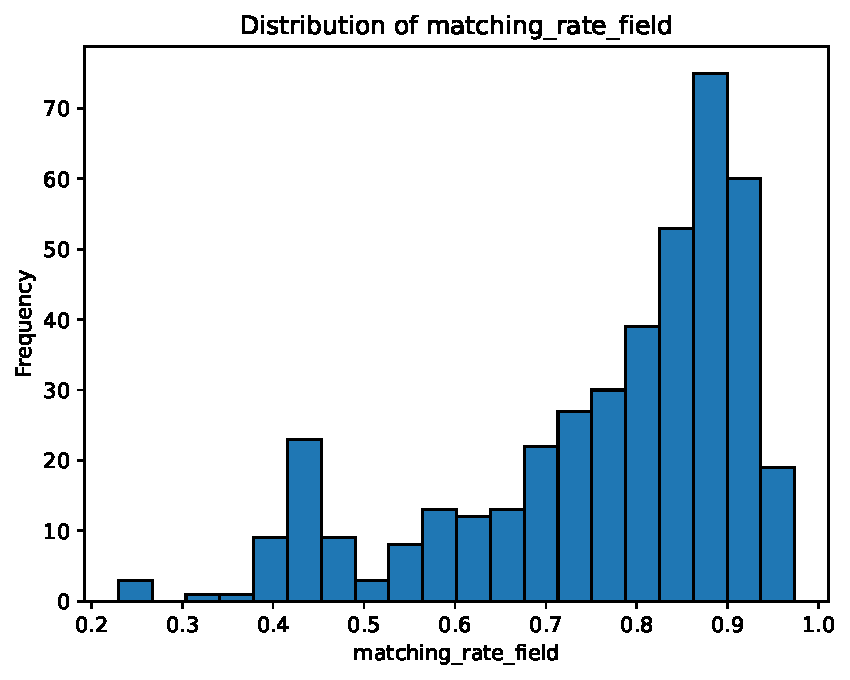
\includegraphics[width=\linewidth]{Images/distribution_matching_rate_field.pdf}
        \caption{Field-level matching rate}
        \label{fig:dist-match-field}
    \end{subfigure}\hfill
        \begin{subfigure}[b]{0.48\linewidth}
        \centering
        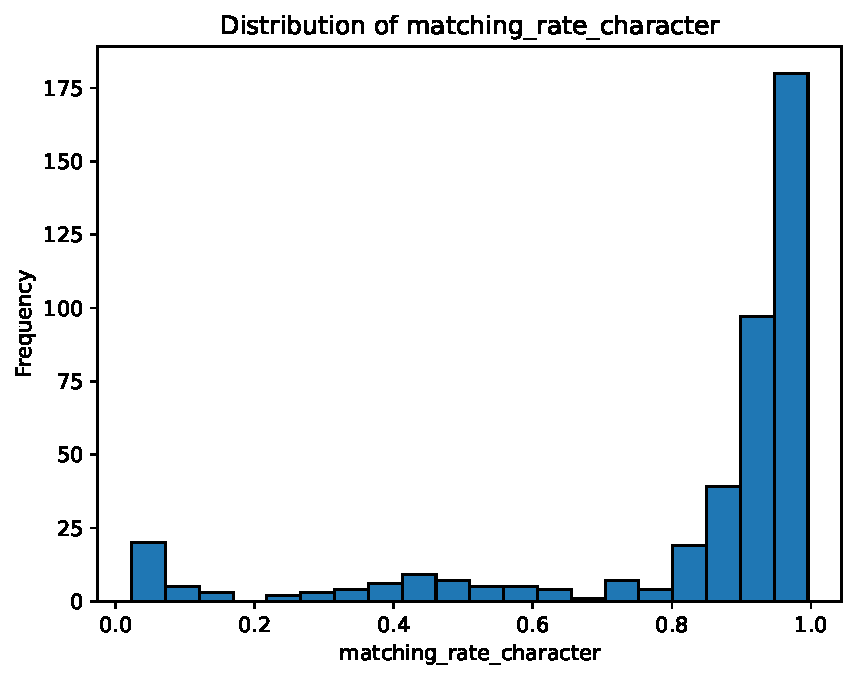
\includegraphics[width=\linewidth]{Images/distribution_matching_rate_character.pdf}
        \caption{Character-level matching rate}
        \label{fig:dist-match-char}
    \end{subfigure}



    \vspace{0.6em}

    \begin{subfigure}[b]{0.48\linewidth}
        \centering
        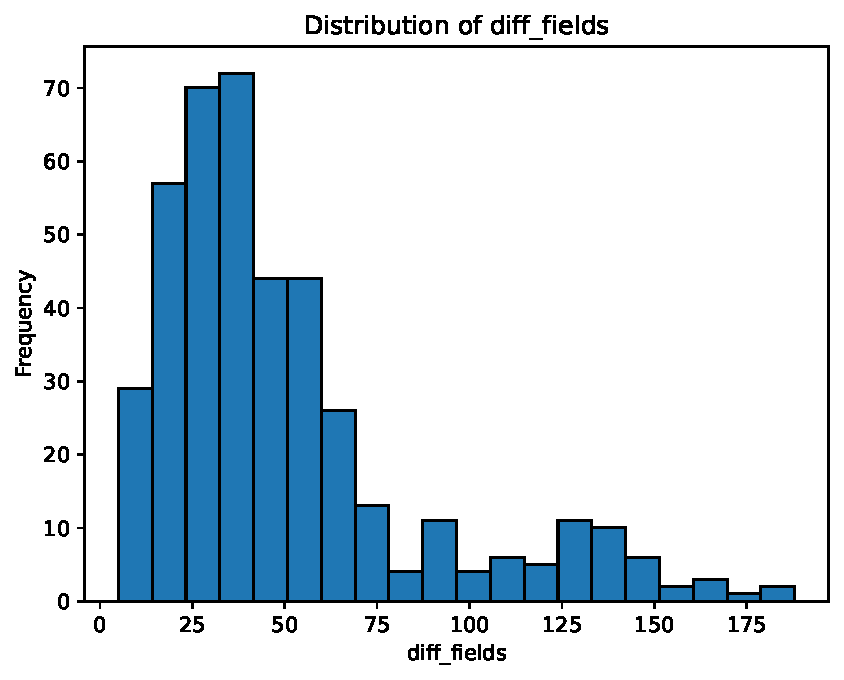
\includegraphics[width=\linewidth]{Images/distribution_diff_fields.pdf}
        \caption{Distribution of different fields}
        \label{fig:dist-diff-fields}
    \end{subfigure}\hfill
    \begin{subfigure}[b]{0.48\linewidth}
        \centering
        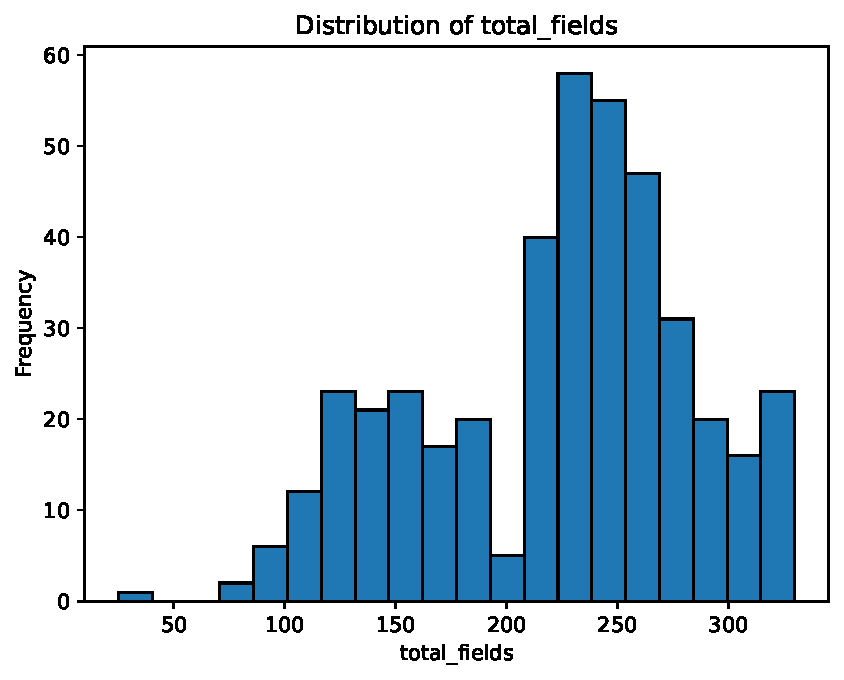
\includegraphics[width=\linewidth]{Images/distribution_total_fields.pdf}
        \caption{Distribution of total fields}
        \label{fig:dist-total-fields}
    \end{subfigure}

    \caption{Distributions of matching rate and fields count over the data 210 columns}
    \label{fig:four-distributions}
\end{figure}


After filtering, we have the 58 columns to serve as the benchmark. The field matching statistics are shown in Figure~\ref{tab:field_iaa_by_pair_cleaned}.

On the second layer of our framework, we have 991 fields to correct, out of 13595 fields in total, which is only 7.2\% human effort. We can still improve the efficiency of our framework by conducting more rule-based automatic review, for example resolve the conflict in address with only the difference like "Marseille" and "à Marseille".

\begin{table}[htbp]
\centering
\caption{Aggregated field-level matching rate by model pair in filtered data}
\label{tab:field_iaa_by_pair_cleaned}
\begin{tabular}{lrrr}
\hline
\textbf{Model pair} & \textbf{Matched fields} & \textbf{Total fields} & \textbf{\% matched fields} \\
\hline
claude\_vs\_qwen & 11,294 & 12,895 & 87.6\% \\
llama\_vs\_grok & 11,048 & 12,905 & 85.6\% \\
\hline
\end{tabular}
\end{table}

\section{Correction Platform}

To facilitate the human correction of the data fields where machines don't reach consensus, we developed an annotation platform. With this platform, our annotator could focus on correcting the different results from machine annotations, as is shown in Figure~\ref{fig:platform}.

We use red box to highlight the fields with different machine annotations, and we also highlight the exact different character in the field. In this way, we exploit the maximum utility of the machine consensus and improve the manual correction efficiency and accuracy.

We have our researcher Ren Yi and Ella Bischoff from UNIL to conduct the human correction. We appreciate their work.

\begin{figure}
    \centering
    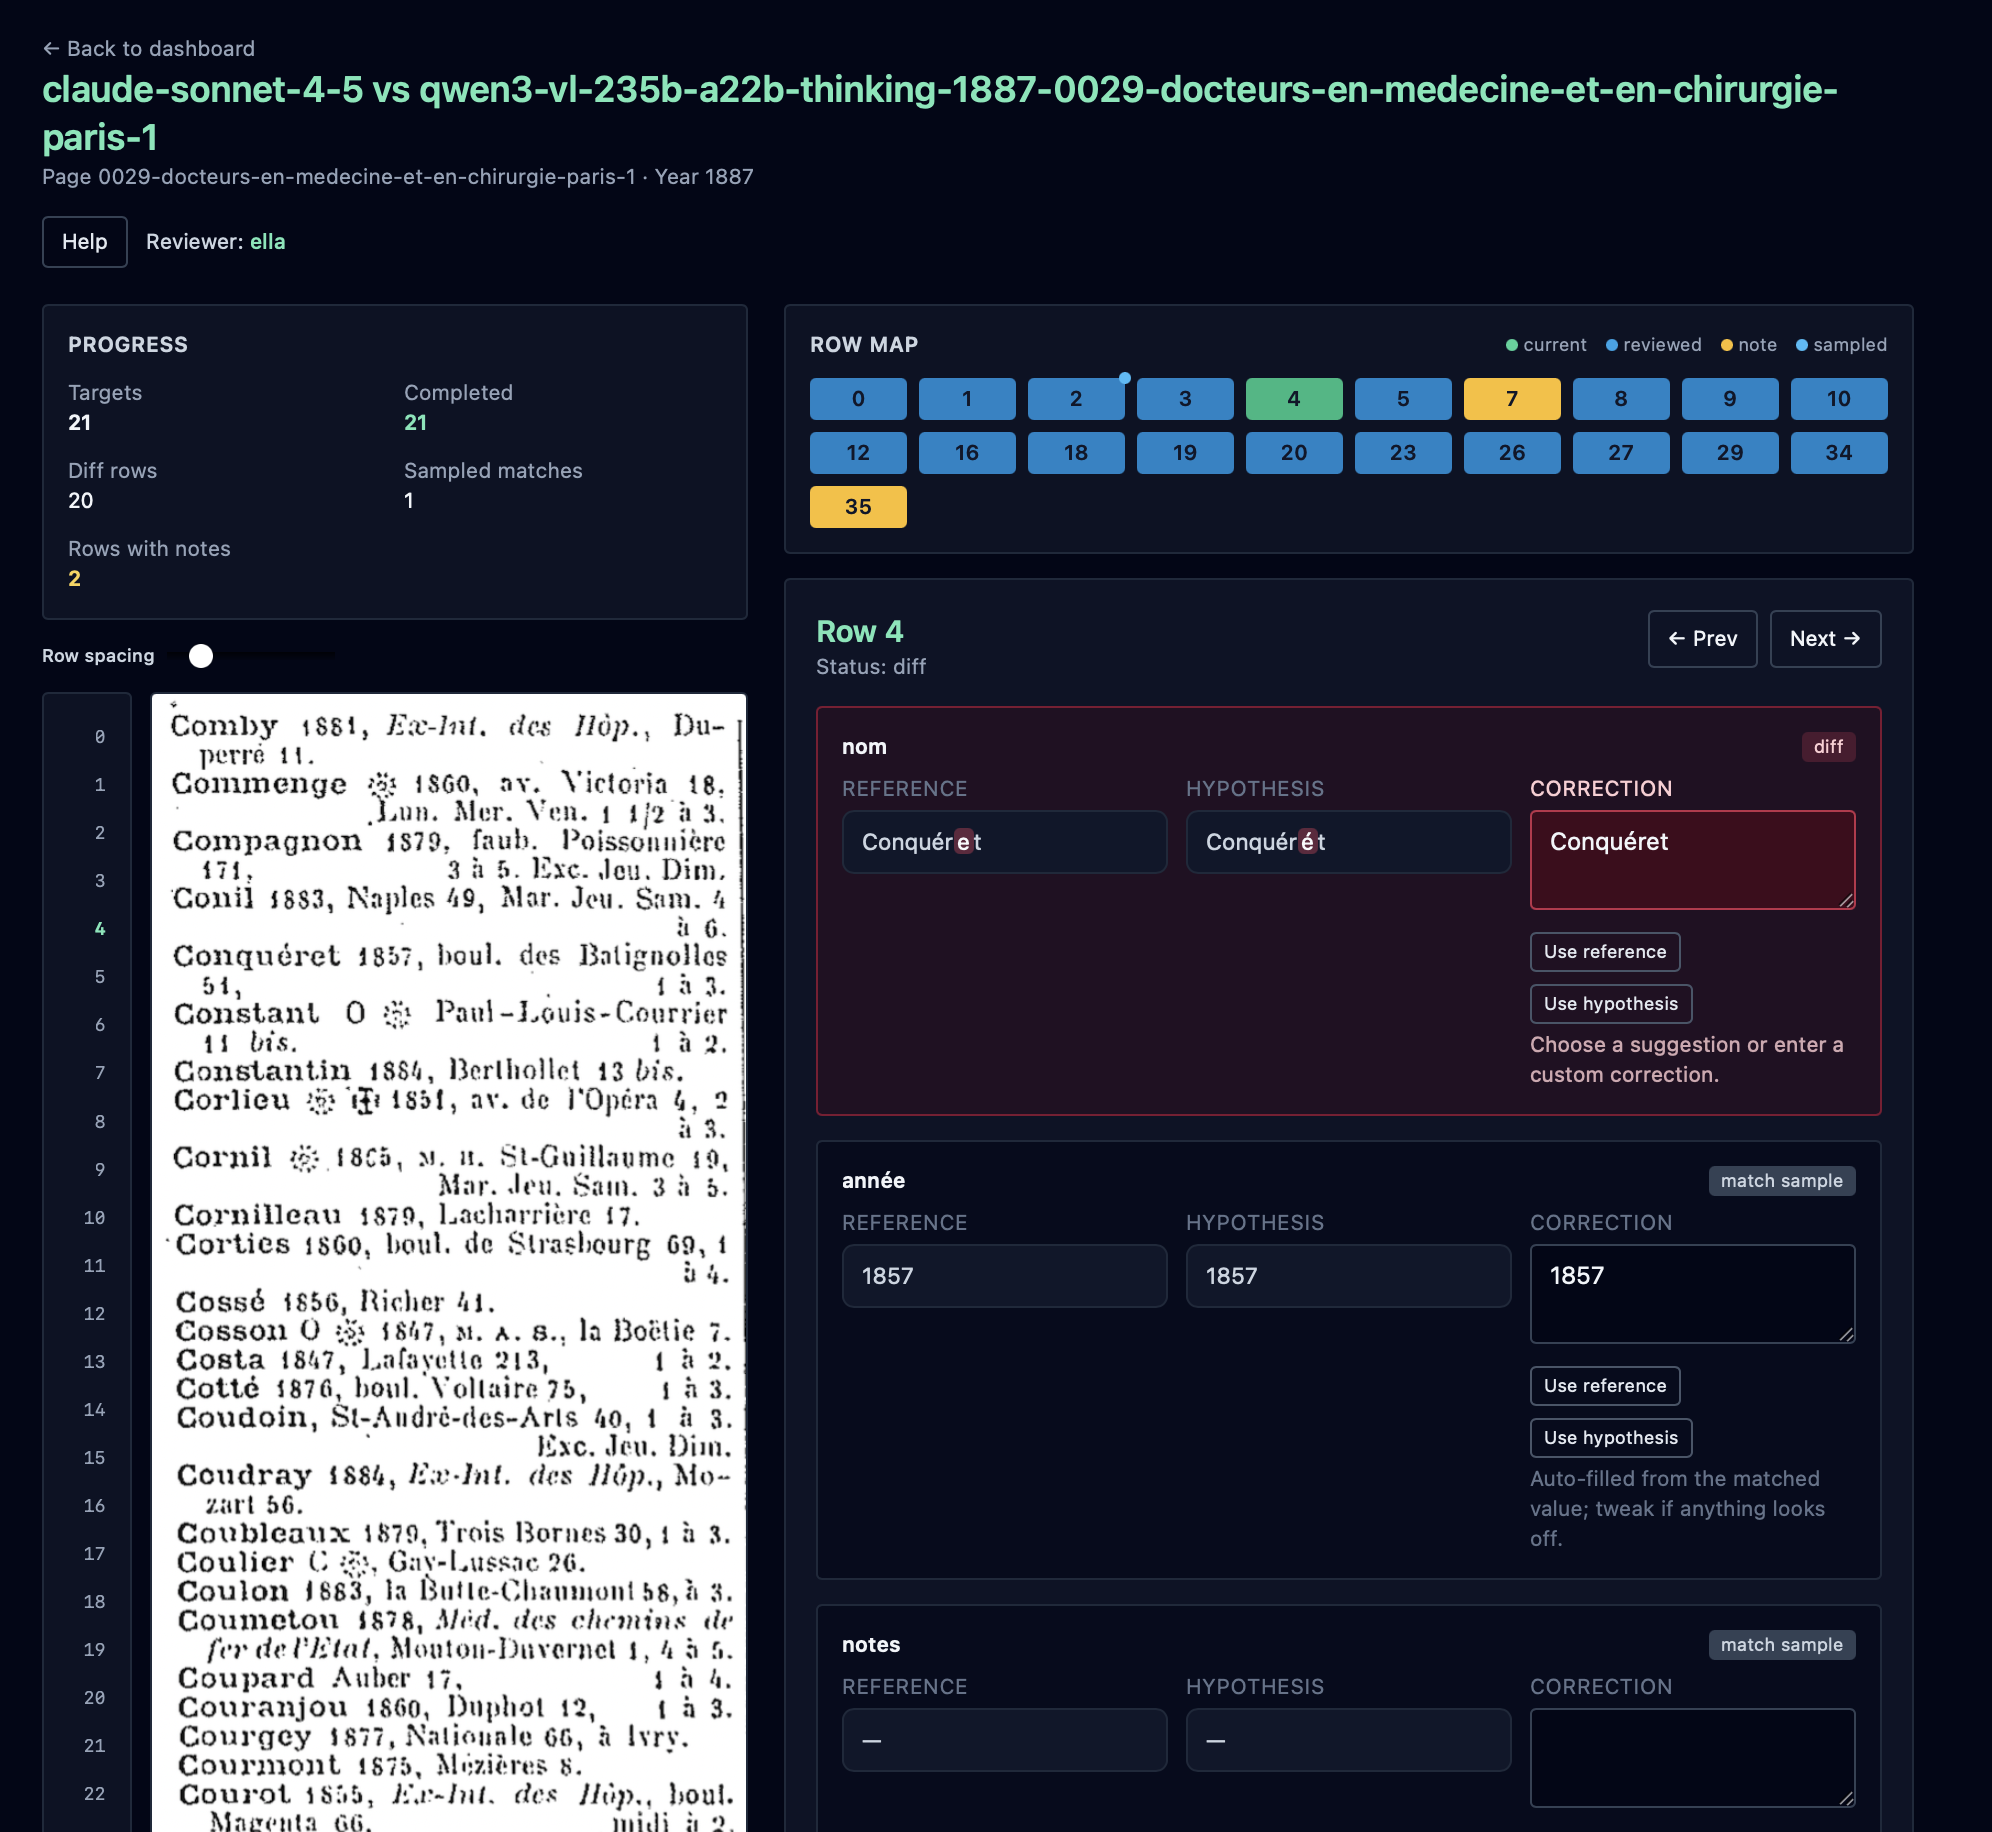
\includegraphics[width=0.8\linewidth]{Images/platform.png}
    \caption{Human Correction Platform}
    \label{fig:platform}
\end{figure}
\section{Image Preprocessing Necessity}
\label{sec:image-preprocessing}
Table~\ref{tab:wer_image_ablation} reports word error rate (WER; lower is better) under four image-input setups: \emph{raw} (baseline), \emph{no-ad} (removing auxiliary ``ad/extra'' content), \emph{split} (splitting the page into columns before inference), and \emph{concat} (concatenating split columns).
Overall, removing auxiliary content is broadly beneficial: \textbf{12/13} models improve from \emph{raw} to \emph{no-ad}, with a median relative WER reduction of \textbf{20.03\%} (mean: 22.27\%).
Splitting is often the most effective downstream strategy: \textbf{split} yields the best WER for \textbf{7/13} models (vs.\ \textbf{5/13} for \emph{no-ad}), and achieves the best absolute result in our runs with \texttt{gemini-3-pro-preview} (\textbf{WER=0.0351}).
In contrast, concatenation is unstable: only \textbf{4/13} models improve under \emph{concat}, while several degrade severely (e.g., Claude models).
Notably, \texttt{gpt-5.1} is an outlier where \emph{no-ad} harms performance (WER 0.1221 $\rightarrow$ 0.1656), but \emph{split} largely recovers accuracy (WER 0.0853).


% Preamble suggestions:
% \usepackage{booktabs}
% \usepackage{graphicx} % for \resizebox

\begin{table}[t]
\centering
\small
\setlength{\tabcolsep}{4pt}
\resizebox{\linewidth}{!}{%
\begin{tabular}{lrrrrrrr}
\toprule
LLM & WER$_{\mathrm{raw}}$ & WER$_{\mathrm{no\text{-}ad}}$ & $\Delta_{\mathrm{raw}\rightarrow\mathrm{no\text{-}ad}}$ (\%) &
WER$_{\mathrm{split}}$ & $\Delta_{\mathrm{no\text{-}ad}\rightarrow\mathrm{split}}$ (\%) &
WER$_{\mathrm{concat}}$ & $\Delta_{\mathrm{no\text{-}ad}\rightarrow\mathrm{concat}}$ (\%) \\
\midrule
claude-haiku-4-5                 & 0.1371 & 0.0987 &  28.01 & 0.0870 &  11.85 & 0.5987 & -506.59 \\
claude-opus-4-1                  & 0.1338 & 0.1070 &  20.03 & 0.1104 &  -3.18 & 0.5151 & -381.40 \\
claude-sonnet-4-5                & 0.1438 & 0.0886 &  38.39 & 0.0836 &   5.64 & 0.5234 & -490.74 \\
gemini-2.5-flash                 & 0.1371 & 0.0870 &  36.54 & 0.0669 &  23.10 & 0.0736 &   15.40 \\
gemini-2.5-pro                   & 0.0652 & 0.0619 &   5.06 & 0.0669 &  -8.08 & 0.0619 &    0.00 \\
gemini-3-pro-preview             & 0.0585 & 0.0552 &   5.64 & 0.0351 &  36.41 & 0.0569 &   -3.08 \\
gpt-5-mini                       & 0.0803 & 0.0753 &   6.23 & 0.0870 & -15.54 & 0.1187 &  -57.64 \\
gpt-5.1                          & 0.1221 & 0.1656 & -35.63 & 0.0853 &  48.49 & 0.2408 &  -45.41 \\
grok-4                           & 0.1923 & 0.1756 &   8.68 & 0.1288 &  26.65 & 0.1589 &    9.51 \\
grok-4-1-fast-reasoning          & 0.9532 & 0.3662 &  61.58 & 0.9097 & -148.42 & 0.9448 & -158.00 \\
llama4-maverick                  & 0.1421 & 0.0920 &  35.26 & 0.0686 &  25.43 & 0.0702 &   23.70 \\
qwen3-vl-235b-a22b-thinking      & 0.0853 & 0.0702 &  17.70 & 0.0719 &  -2.42 & 0.0736 &   -4.84 \\
qwen3-vl-8b-thinking             & 0.3478 & 0.1321 &  62.02 & 0.1405 &  -6.36 & 0.1120 &   15.22 \\
\bottomrule
\end{tabular}%
}
\caption{WER ablation across image-input strategies. Positive $\Delta$ indicates a relative WER reduction (improvement) versus the reference configuration.}
\label{tab:wer_image_ablation}
\end{table}


\paragraph{Best strategy for the selected models.}
For our selected models, we choose the image-input configuration that minimizes WER (Table~\ref{tab:wer_image_ablation}).
For \texttt{claude-sonnet-4-5}, \textbf{split} performs best (WER=0.0836), improving over \emph{no-ad} (0.0886), whereas \emph{concat} degrades substantially (0.5234).
For \texttt{qwen3-vl-235b-a22b-thinking}, \textbf{no-ad} is marginally best (WER=0.0702); \emph{split} (0.0719) and \emph{concat} (0.0736) yield no further gains.
For \texttt{llama4-maverick} and \texttt{grok-4}, \textbf{split} is clearly optimal (WER=0.0686 and 0.1288, respectively), suggesting that region-wise processing is beneficial for these models.
In summary, \textbf{split} is optimal for \textbf{3/4} selected models and is within 0.0017 WER of the best setting for the remaining one; for consistency across systems, we therefore adopt \textbf{split} for all four models.

Particularly, the dramatic performance drop with the strategy concat, could result from the too long image after concatenation, Claude 4.5 Sonnet would be scaled down before converting to tokens \footnote{https://platform.claude.com/docs/en/build-with-claude/vision}, which could degrate the performance significantly. 

\section{Conclusion}
This chapter constructs a representative benchmark from the Rosenwald Guides via stratified sampling and creates annotations using a double-layer framework: two independent MLLM systems produce initial TSV outputs. After post-filtering to prioritize high-consensus and feasible cases, we obtain a 60-column benchmark in which model agreement exceeds 85\%. In the final review layer, we only need to manually correct 991 fields out of 13595, and this efficiency could be further improved. Finally, an ablation study shows that removing ads and splitting pages into columns consistently improves OCR quality, motivating the use of \textit{split} preprocessing across our selected models.
